\section{Experimental Results} 
\label{sec:results}

\subsection{Experimental Setup}

Our design is described in HLS C and synthesized using the Vivado HLS \cite{HLS2011}.
The accelerator engine contains two PE arrays, each composed of 50 PEs, and can run at 150MHz on the Xilinx VC707 FPGA evaluation board.
The FPGA resource utilization is approximately 65\% (LUT: 65.4\%, Reg: 30.7\%). 
We use an input with 100M reads, which is a subset collected from a real individual human genome sample (about 500M reads, 120GB FASTQ file) with breast cancer (HCC1954). 
We verify the outputs of our FPGA implementation with the seed extension step of BWA-MEM to ensure correctness. 

\subsection{Speedup Over Software-Based BWA-MEM}

To demonstrate the speedup of our accelerator engine over the original BWA-MEM software, 
an Intel Haswell Xeon server with two 6-core CPUs is used.
The server can run 24 threads in parallel, with hyperthreading support.
We compare the execution time of our FPGA implementation with pure software-customized S-W runtimes with 1, 2, 4, 8, 16 and 24 threads, respectively.
To make it a fair comparison, only the computation time of the S-W calls (after loading inputs from memory and before storing outputs to memory) is collected for both FPGA and CPU implementations.

Figure \ref{fig:F1C5} shows the performance comparison between our FPGA design and the software BWA-MEM S-W kernel with results normalized to the single-threaded CPU performance.
Our FPGA design outperforms the 24-thread CPU by 26.4 times.

\subsection{Speedup Over Wavefront-Based Designs}

To highlight the advantage of our design over wavefront-based solutions, 
we compare the runtime of our accelerator engine to those of a set of wavefront-based FPGA implementations described in \cite{Zhang2007}. To arrive at a fair comparison, we try to implement all designs with roughly the same FPGA resource utilization.

Table \ref{tab:configuration} shows the wavefront-based designs that we implemented for comparison. 
A design containing $n$ kernels with $m$ PE per kernel is denoted by $m$Px$n$K. 
We use the 32Px5K configuration as the base unit for comparison.
We find that the performance of the wavefront-based designs generally decreases when the number of PEs per kernel ($m$) increases.
although the performance does not decrease fully monotonically, as shown in Figure \ref{fig:F2C5}.
In general, this verifies that the wavefront-based designs have worse PE utilization rates compared to our design. 

\begin{figure}[!hbt]
	\begin{center}
		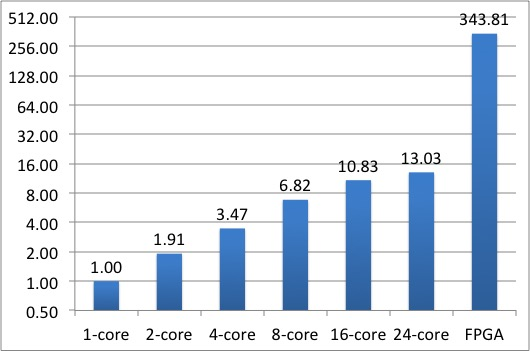
\includegraphics[width=2.5in]{Figures/F1C5.jpg}
		\caption {Performance comparison between our FPGA design and the multi-threaded BWA-MEM software in doing S-W. A base-2 logarithmic scale is used for the Y axis to denote the normalized performance.}
		\label{fig:F1C5}
	\end{center}
\end{figure}
\vspace{-20pt}

%%%\vspace{-2pt}
\begin{figure}[!hbt]
	\begin{center}
		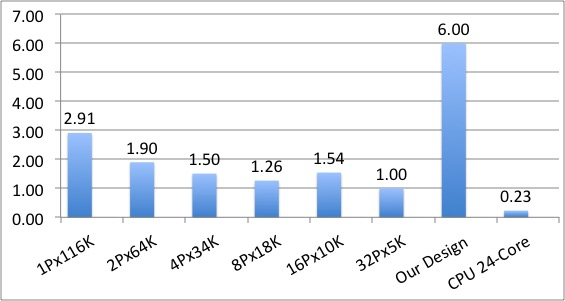
\includegraphics[width=2.5in]{Figures/F2C5.jpg}
		\caption {Performance comparison between our design and a set of wavefront-based designs. The Y axis denotes the performance normalized to that of the 32Px5K configuration.}
		\label{fig:F2C5}
	\end{center}
\end{figure}
\vspace{-10pt}

Furthermore, Figure \ref{fig:F2C5} also demonstrates the power of pruning. 
When the wavefront design goes to the extreme where a kernel is restricted to have only one PE (1Px116K), 
the only difference between our design and the 1Px116K design is whether the pruning logics are realized. 
Compared to the 1Px116K design, our design shows about 2x speedup.
%%% even though the number of PEs in our design is only 100, which is 16 PEs fewer than that of 1Px116K. 
Our current design uses reads with a length of 101bp.
Since the trend of NGS will generate longer reads in the future, the performance improvement lead by pruning is expected to be much more significant.
%%%
%%%We need to mention that resources can be saved when more PEs are integrated into one kernel for the wavefront-based designs.
%%%First, the PEs in one kernel can share one copy of control logics. A design with a large number of kernels spends more resources on the control logics.
%%%Moreover, for the wavefront implementations, the logics for pruning are not required.
%%%That is why the 32Px5K design can contain 60\% more PEs than that of our design.
%%%\subsection{The Effectiveness of Pruning}
%%%\subsection{The Need for Two-Level Scheduling}
%%%
%%%%We find that the efficiency of the task distributor can potentially become the performance bottleneck 
%%%%since the sequential round-robin scheduling becomes the critical path when the number of PEs in a PE array increases.
%%%%Compared to our accelerator engine with two PE arrays, the performance of the single PE array design is 38.9\% worse.
%%%%Both of them have 100 PEs in total.
%%%
%%%The efficiency of the task distributor can potentially become the performance bottleneck.
%%%Figure \ref{fig:F3C5} shows the performance of a PE array with different numbers of PEs.
%%%Before the number of PEs in a PE array reaches a threshold,
%%%the performance can scale almost linearly proportional to the number of PEs.
%%%The performance of a PE array scales poorly when the number of PEs is larger than 50 in our design.
%%%Therefore, to optimize system performance, our accelerator engine uses two-level scheduling and thus has two PE arrays. 
%%%Each PE array contains 50 PEs. The FPGA resource constraint prevents us from adding more PE arrays.
%%%
%%%\begin{figure}[!hbt]
%%%	\begin{center}
%%%		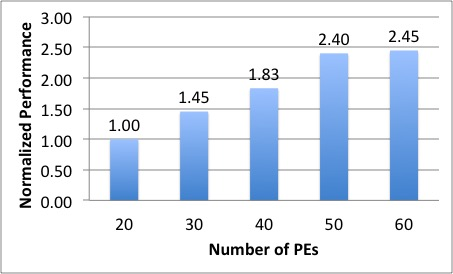
\includegraphics[width=2.8in]{Figures/F3C5.jpg}
%%%		\caption {The performance scalibility of a PE array with different numbers of PEs.}
%%%		\label{fig:F3C5}
%%%	\end{center}
%%%\end{figure}
